\model{The ``Vee'' Tree}

Open \textit{VeeTree.java} and run the program.
Adjust the \java{DELAY} in \textit{Drawing.java}, as needed, to notice the order.
Then answer the questions below to explore and discuss the source code as a team.

\begin{multicols}{2}

\begin{center}
\textbf{Drawing (cropped)}
\end{center}

\fbox{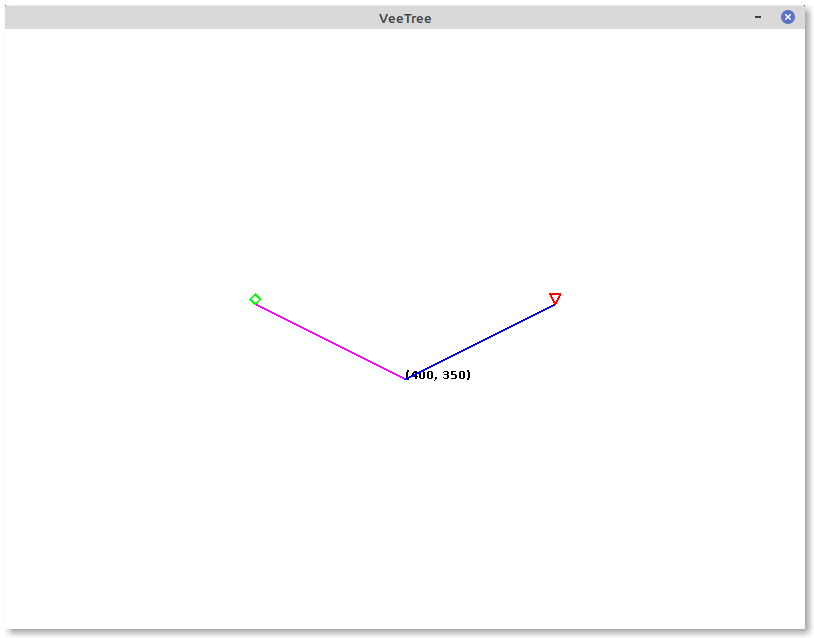
\includegraphics[trim=200 175 200 175,clip,width=\linewidth]{VeeTree.png}}

\columnbreak

\begin{center}
\textbf{Console output}
\end{center}

\vspace{-1em}

\begin{javalst}
  Starting vee(400, 350)
  diamond(250, 275)
  triangle(550, 275)
  Finished vee(400, 350)
\end{javalst}

\end{multicols}


\quest{15 min}


%\Q What type of object is constructed in the \java{main} method?
%%
%\hfill \ans[16em]{A \jans{VeeTree} (which IS-A \jans{Drawing})}


%\Q Explain how the \java{main} method calls the \java{Drawing()} constructor.
%
%\begin{answer}
%\textit{VeeTree.java} does not define any constructors, so the compiler automatically generates one.
%By default, a constructor automatically calls \jans{super()}.
%Since VeeTree extends Drawing, the \jans{Drawing()} constructor is called.
%\end{answer}


\Q The \java{vee()} method uses \java{g2} to draw strings and lines.
Where is this variable declared?

\begin{answer}[2em]
In \textit{Drawing.java}; it's an inherited attribute.
\end{answer}


\Q Review the Javadoc comment for the \java{vee()} method.
In terms of its variables, what are the following coordinates?

\setlength{\defaultwidth}{4em}

\begin{enumerate}
\item The bottom of the ``Vee'': (\ans{x} ~, \ans{y} ~)
\item The diamond on the left:   (\ans{left} ~, \ans{top} ~)
\item The triangle on the right: (\ans{right} ~, \ans{top} ~)
\end{enumerate}


\Q Add the following line at the end of the left branch, after the \java{trace} for diamond.
What happens when you run the program now?
Explain both the drawing and the Console output.

\begin{javalst}
vee(level + 1, left, top);
\end{javalst}

\begin{answer}[5em]
The left branch continues drawing ``forever'' (until a \jans{StackOverflowError}).
Based on the output, the \java{vee} method calls itself repeatedly with an increasing \jans{level} each time.
\end{answer}


\newpage

\Q Add the following code at the beginning of the method, right after the first \java{trace}.
What happens when you run the program now?
Explain both the drawing and the Console output.

\begin{javalst}
if (level == 3) {
    trace(level, "Aborting vee(%d, %d)", x, y);
    return;
}
\end{javalst}

\begin{answer}[5em]
The program draws a ``Vee'' shape at the top of each left branch, but it stops after 3 levels to avoid going on forever.
The output increases to level 3, and then it decreases back to level 0.
\end{answer}


\Q Based on the most recent Console output:

\setlength{\defaultwidth}{1.5em}

\begin{multicols}{2}
\begin{enumerate}
\item How many times was \java{vee()} called? \ans{4}
\item How many times did \java{vee()} return? \ans{4}
\item How many diamonds were drawn? \ans{3}
\item How many triangles were drawn? \ans{3}
\end{enumerate}
\end{multicols}


\Q \label{key2}
Add the following line at the end of the right branch, after the \java{trace} for triangle.
What happens when you run the program now?
Explain both the drawing and the Console output.

\begin{javalst}
vee(level + 1, right, top);
\end{javalst}

\begin{answer}[5em]
The drawing is now symmetrical---there is a ``Vee'' shape at the top of each branch.
Along the top of the drawing, there are eight branches that abort the recursion.
The output both increases and decreases in level as the drawing moves up and down.
\end{answer}
